% Text-conditioned DiT-S/4 on MS-COCO -- final report (NeurIPS format, nips15submit_e.sty)
% Compile from this folder: references.bib and the figures in outputs/ are stored next to this file.
\documentclass{article}
\usepackage{nips15submit_e,times}
\nipsfinalcopy

\usepackage[utf8]{inputenc}
\usepackage[T1]{fontenc}
\usepackage{amsmath,amssymb}
\usepackage{graphicx}
\usepackage{booktabs}
\usepackage{xcolor}
\usepackage{url}
\usepackage[hidelinks]{hyperref}

\newcommand{\todo}[1]{\textcolor{red}{[TODO: #1]}}
\newcommand{\nullemb}{\varnothing}
\newcommand{\epooled}{e_{\mathrm{pooled}}}
\newcommand{\temb}{t_{\mathrm{emb}}}
\newcommand{\yemb}{y_{\mathrm{emb}}}

\title{Text-conditioned DiT-S/4 on MS-COCO}

\author{
Linda Fei Payeras Olano \\
Universidad Aut\'onoma de Madrid \\
{\small\texttt{linda.payeras@estudiante.uam.es}} \And
Milagros Rodriguez Ventura \\
Universidad Aut\'onoma de Madrid \\
{\small\texttt{milagros.rodriguez@estudiante.uam.es}} \AND
David L\'opez Valdivia \\
Universidad Aut\'onoma de Madrid \\
{\small\texttt{david.lopezvaldivia@estudiante.uam.es}} \And
Daniel Cruz Navarro \\
Universidad Aut\'onoma de Madrid \\
{\small\texttt{daniel.cruzn@estudiante.uam.es}}
}

\begin{document}
\maketitle

% ---------------------------------------------------------------------------
\begin{abstract}
Diffusion Transformers (DiT) replace the convolutional U-Net of latent diffusion models with a Vision Transformer, but the original DiT is conditioned only on ImageNet class labels.
We adapt the smallest configuration, DiT-S/4, to text-conditioned generation on MS-COCO Captions.
Captions are encoded by a frozen CLIP ViT-L/14 text encoder, and the pooled vector $\epooled$ is projected by a small MLP and added to the timestep embedding, so that every block regresses its adaLN-Zero modulation with a global channel-wise shift and scale.
The final run trained on 45,174 COCO train2014 images containing people, with a person-centered crop, batch 128 and 150,000 steps on CPU, with an all-zero null embedding $\nullemb$.
On 10K unfiltered val2014 images with a center crop, classifier-free guidance improves both metrics up to $s=4$ (FID-10K 71.2168, CLIP Score ViT-L/14 18.2717 with DPM-Solver++ 20 steps), and at $s=5$ CLIP Score still rises while FID-10K worsens.
Image quality remains limited: scenes and colors relate to the caption, but objects and people are deformed.
Results are better on validation images with person annotations than without; we describe this difference but do not establish its cause.
\end{abstract}

% ---------------------------------------------------------------------------
\section{Introduction}

Latent diffusion models generate images by learning to reverse a gradual noising process in the latent space of a pretrained autoencoder~\cite{ho2020ddpm,rombach2022ldm}.
Peebles and Xie~\cite{peebles2023dit} showed that the denoising network can be a plain transformer operating on patches of the latent (DiT), and that its sample quality improves with model size and width.
Their models are conditioned on a discrete ImageNet class label through adaptive layer normalization with zero-initialized gates (adaLN-Zero).

This project adapts DiT from class-conditional to text-conditional generation.
A class label is a lookup into a table of 1,001 learned embeddings; a caption must instead be encoded into a continuous vector and projected to the model width.
We keep the DiT backbone, the diffusion process and the hybrid loss unchanged, and replace the label embedder with a text embedder that takes the pooled output of a frozen CLIP text encoder~\cite{radford2021clip}.
Because the caption enters only through the global adaLN-Zero modulation, the caption is never attended to by image tokens; we call this conditioning adaLN-Zero-Text.

We train the smallest DiT configuration, DiT-S/4, on MS-COCO Captions~\cite{lin2014coco} and evaluate it with FID-10K and CLIP Score across classifier-free guidance (CFG) scales.
The run that was completed differs from the original specification in data, crop, batch size, training length, hardware and null embedding; we report these deviations explicitly (Table~\ref{tab:deviations}).

% ---------------------------------------------------------------------------
\section{Objectives}

\begin{enumerate}
  \item Build an offline pipeline that pre-extracts VAE latent statistics and frozen CLIP pooled text embeddings from MS-COCO Captions, and serves them to training through a memory-mapped dataset.
  \item Implement adaLN-Zero-Text conditioning in DiT-S/4: a text embedder for $\epooled$, a frozen null embedding $\nullemb$ with 15\% text dropout, and classifier-free guidance on all four noise channels.
  \item Train the model and evaluate fidelity (FID-10K) and text--image alignment (CLIP Score) across CFG scales $s\in\{1,1.5,2,3,4,5\}$ with DPM-Solver++ (20 steps), and with DDPM (250 steps) at the best guidance scale.
  \item Document the work in a public repository with tests and a tutorial notebook, and report deviations from the specification and the limits of the evidence.
\end{enumerate}

% ---------------------------------------------------------------------------
\section{Related work and state of the art}

\paragraph{Diffusion models.}
Denoising diffusion probabilistic models (DDPM)~\cite{ho2020ddpm} train a network $\epsilon_\theta$ to predict the noise added to data and generate samples by iterative denoising.
Nichol and Dhariwal~\cite{nichol2021improved} additionally learn the reverse-process variance $\Sigma_\theta$ through a hybrid objective $L_{\mathrm{simple}}+\lambda L_{\mathrm{vlb}}$, which allows sampling with a learned variance schedule.
DPM-Solver++~\cite{lu2022dpmsolverpp} is a high-order solver for guided sampling that produces samples in around 20 steps.
Classifier-free guidance~\cite{ho2022cfg} trains a single model both with and without the condition and, at sampling time, extrapolates from the unconditional towards the conditional prediction, traditionally improving text alignment at the cost of image fidelity.

\paragraph{Latent diffusion and transformer backbones.}
Latent diffusion models~\cite{rombach2022ldm} run the diffusion process in the latent space of a pretrained autoencoder, which reduces cost, and condition a U-Net on text through cross-attention.
DiT~\cite{peebles2023dit} replaces the U-Net with a transformer over latent patches; the paper compares in-context conditioning, cross-attention and adaptive layer norm, and adopts adaLN-Zero for class conditioning.
Esser et al.~\cite{esser2024sd3} use a pooled CLIP text vector, processed by an MLP, as a global conditioning signal combined with the timestep embedding in a transformer-based text-to-image model; our approach follows the same global-conditioning logic while keeping the original DiT block structure.
Other transformer backbones have also been applied to text-to-image diffusion.
U-ViT~\cite{bao2023uvit} treats the time, the condition and the noisy image patches all as tokens, adds long skip connections between shallow and deep layers, and reports text-to-image results on MS-COCO.
PixArt-$\alpha$~\cite{chen2023pixartalpha} incorporates cross-attention modules into DiT to inject text conditions and reports a training cost of about 10.8\% of the GPU time of Stable Diffusion v1.5.
Unlike these models, ours keeps the DiT block unchanged and injects text only through the global adaLN-Zero modulation.

\paragraph{Text encoders and evaluation.}
CLIP~\cite{radford2021clip} learns aligned image and text embeddings contrastively; its pooled text output is trained to summarize a caption in a single vector, which makes it a natural input to global conditioning.
Fr\'echet Inception Distance (FID)~\cite{heusel2017fid} compares the statistics of Inception features of real and generated sets; clean-fid~\cite{parmar2022cleanfid} standardizes resizing and implementation details.
CLIPScore~\cite{hessel2021clipscore} measures image--text compatibility as a scaled cosine similarity of CLIP embeddings.

% ---------------------------------------------------------------------------
\section{Methodology}

\subsection{Latent space, text encoder and data pipeline}

Images of size $256\times256\times3$ are encoded by the frozen Stable Diffusion VAE \texttt{sd-vae-ft-ema}~\cite{stability_sdvae} (downsampling $f=8$) into latents $z_0\in\mathbb{R}^{4\times32\times32}$.
The same VAE is used for encoding and decoding.
Captions are tokenized to 77 tokens and encoded by the frozen CLIP ViT-L/14 text encoder; we use its pooled [EOS] output $\epooled\in\mathbb{R}^{768}$.
The token sequence $E_{\mathrm{seq}}$ is not stored, since only a cross-attention variant would use it.

Because VAE and CLIP are frozen, their outputs are computed once, offline.
For every training image and its horizontal flip we store the posterior mean and standard deviation of the VAE (unscaled, fp16), and for each of its five captions we store $\epooled$.
The dataset memory-maps these arrays and, for each item, draws a flip and one of the five captions at random and samples a fresh latent $z_0=(\mu+\sigma\odot\eta)\cdot0.18215$, $\eta\sim\mathcal{N}(0,\mathbf{I})$.

\subsection{DiT-S/4 with adaLN-Zero-Text}

DiT-S/4 has 12 blocks, width $d=384$, 6 attention heads and patch size $p=4$, giving 64 tokens from a $32\times32$ latent.
The model has \texttt{learn\_sigma=True} and outputs 8 channels: $\epsilon_\theta$ (4) and $\Sigma_\theta$ (4); the total parameter count is 33,003,776.
We replace DiT's class-label lookup table with a \emph{text embedder}, a two-layer MLP (Linear $768\to384$, SiLU, Linear $384\to384$) with the same structure as the timestep embedder:
\begin{equation}
  \yemb=\mathrm{MLP}(\epooled),\qquad c=\temb+\yemb\in\mathbb{R}^{384}.
\end{equation}
Each block maps $c$ through SiLU and a linear layer to six vectors $(\beta_1,\gamma_1,\alpha_1,\beta_2,\gamma_2,\alpha_2)$ and computes
\begin{align}
  x &\leftarrow x+\alpha_1\odot\mathrm{Attn}\big(\mathrm{LN}(x)\odot(1+\gamma_1)+\beta_1\big),\\
  x &\leftarrow x+\alpha_2\odot\mathrm{MLP}\big(\mathrm{LN}(x)\odot(1+\gamma_2)+\beta_2\big).
\end{align}
The same modulation applies to all 64 tokens: the caption scales and shifts feature channels globally and is never attended to; spatial layout must emerge from self-attention among image tokens.
The gates $\alpha$ are zero-initialized, so every block starts as the identity (adaLN-Zero) and the model output is zero at initialization, which we verified.
All other DiT components (patch embedding, 2D sine-cosine positional embedding, timestep embedder, blocks, final layer and diffusion code) are reused unchanged.

\subsection{Training objective, CFG and sampling}

The forward process uses $T=1000$ steps with a linear schedule $\beta_t$ from $10^{-4}$ to 0.02, and $z_t=\sqrt{\bar\alpha_t}\,z_0+\sqrt{1-\bar\alpha_t}\,\epsilon$.
We use the hybrid loss of DiT~\cite{nichol2021improved,peebles2023dit},
\begin{equation}
  L=L_{\mathrm{simple}}+L_{\mathrm{vlb}},\qquad L_{\mathrm{simple}}=\mathbb{E}\,\big\|\epsilon-\epsilon_\theta(z_t,t,c)\big\|^2,
\end{equation}
where the MSE term trains $\epsilon_\theta$ and the variational term trains $\Sigma_\theta$ (with a stop-gradient on the mean).
As implemented in the DiT code, the two terms are added directly, with no additional weight on $L_{\mathrm{vlb}}$, which is measured in bits per dimension.
Weights are averaged with an exponential moving average (EMA) of decay 0.9999, and the EMA weights are used for all sampling and evaluation.

For classifier-free guidance~\cite{ho2022cfg}, 15\% of training captions are replaced by a null embedding $\nullemb$ (measured rate 0.1501 over 100,000 draws).
At sampling time, the conditional and unconditional predictions are computed in one doubled batch and combined as
\begin{equation}
  \hat\epsilon=\epsilon_\theta(z_t,t,\nullemb)+s\,\big(\epsilon_\theta(z_t,t,\epooled)-\epsilon_\theta(z_t,t,\nullemb)\big).
\end{equation}
The original DiT code guides only three of the four latent channels for reproducibility of its published numbers; we apply guidance to all four $\epsilon$ channels, and leave $\Sigma_\theta$ unguided.
Our default sampler is DPM-Solver++~\cite{lu2022dpmsolverpp} (second-order multistep, 20 steps) configured with the training schedule; the alternative is the DDPM sampler of the DiT code with 250 steps.
DPM-Solver++ is deterministic and ignores $\Sigma_\theta$.

\subsection{Final training run}

The specification planned 82,783 train2014 images with a center crop, batch 256 and 400K steps on a GPU, with $\nullemb$ set to the frozen CLIP embedding of the empty caption.
The single completed run deviates from it as summarized in Table~\ref{tab:deviations}.
It trained on the 45,174 train2014 images that have at least one person box and five captions.
Each crop starts from the union of person boxes with a 20\% margin, is expanded to a square, clipped to the image and resized (bicubic) to 256, so crops clipped at an image border are not square and their aspect ratio changes.
Training used AdamW (learning rate $10^{-4}$, weight decay 0, no warmup, no gradient clipping), global batch 128 and 150,000 steps ($\approx$425 epochs), with bf16 autocast on the model forward only.
$\nullemb$ remained all zeros; sampling and evaluation take $\nullemb$ from the checkpoint, so training, sampling and evaluation use the same all-zero null vector.
Every 10K steps the script saved a checkpoint and a grid of 8 fixed prompts (EMA, DPM-Solver++ 20 steps, $s=4$, seed 0).
The full configuration is listed in Appendix~\ref{app:config}.
COCO train2014 is used for training and val2014 for evaluation, so evaluation images are unseen.

\begin{table}[t]
  \caption{Deviations of the final run from the original specification.}
  \label{tab:deviations}
  \centering
  \small
  \begin{tabular}{@{}lll@{}}
    \toprule
    Item & Specification & Final run \\
    \midrule
    Training images & COCO train2014, 82,783 & 45,174 with $\geq$1 person box and 5 captions \\
    Crop & Center crop of the full image & Square around person boxes $+$20\% margin \\
    Global batch & 256 & 128 \\
    Training length & 400K steps & 150K steps \\
    Seen samples & $\approx$1,237 epochs (102.4M) & $\approx$425 epochs (19.2M, 18.8\% of plan) \\
    Hardware & RTX 3090 & CPU (AVX-512 BF16), $\approx$2.0 steps/s, $\approx$21 h \\
    Null embedding $\nullemb$ & Frozen CLIP(\texttt{""}) & All-zero vector $(1,768)$ \\
    Data loading & Distributed sampler & Single process, shuffled data loader \\
    FID-2K & At 50K, 100K and 150K & At 150K only \\
    \bottomrule
  \end{tabular}
\end{table}

\subsection{Evaluation protocol}

\paragraph{Test set.}
We evaluate on 10K val2014 images.
We sort the image IDs, shuffle them with seed 0 and keep the first 10K, without filtering for people.
Each image is paired with its first caption.
Real and generated images use a 256 center crop.

\paragraph{Generation.}
We use the EMA checkpoint at step 150K to generate one image per caption, using one seed (each batch of 8 uses the index of its first image as its seed).
Generation ran on Apple Silicon (MPS).
We test DPM-Solver++ with 20 steps at $s\in\{1,1.5,2,3,4,5\}$, and DDPM with 250 steps at $s=4$, the scale with the lowest FID in the sweep.

\paragraph{Metrics.}
We compute FID-10K with clean-fid~\cite{parmar2022cleanfid}.
FID values from different sample sizes cannot be compared, and none of our values can be compared with those of the DiT paper.
We compute CLIP Score~\cite{hessel2021clipscore} with torchmetrics as $\max(\mathrm{mean}(100\cos(\mathrm{image},\mathrm{text})),0)$.
Our main metric uses CLIP ViT-L/14, the same model family as the text encoder, and ViT-B/32 serves as a secondary check.

\paragraph{Additional analyses.}
Two further analyses reuse the images generated with DPM-Solver++ 20 at $s=4$, so no new images are generated.
The first computes the CLIP Score of the real images with the same captions.
The second compares metrics between two equal-sized groups of validation images, with and without person annotations.

The repository also includes a tutorial notebook (\path{notebooks/text_to_image_tutorial.ipynb}) that shows the implemented functionality step by step.
% ---------------------------------------------------------------------------
\section{Results and discussion}

\subsection{Training}

The training loss fell from 0.5205 at step 100 to a mean of 0.1687 over steps 140K--150K, with final logged values loss 0.1684, MSE 0.1614 and vb 0.0071 at step 150,000 (Appendix~\ref{app:curve}).
No NaN was logged, and the largest gradient norm was the first (1.40 at step 100).
A falling loss shows that training progressed, not that the model converged.
FID-2K was evaluated only at 150K (94.1912 with DPM-Solver++ 20, $s=4$), so we have no convergence curve.

\subsection{Quantitative results}

Table~\ref{tab:main} and Figure~\ref{fig:cfg} report FID-10K and CLIP Score for the seven configurations.
In this protocol, raising $s$ from 1 to 4 lowers FID-10K from 98.4370 to 71.2168 and raises both CLIP Scores.
At $s=5$ CLIP Score still rises, while FID-10K worsens to 73.2326.
At $s=4$, DPM-Solver++ 20 has a lower FID-10K than DDPM 250, and their CLIP Scores are close.
With a single seed, the 0.76 FID gap between $s=3$ and $s=4$ should not be read as a clear advantage of $s=4$.
A control run of the evaluation code reproduced the FID-10K and both CLIP Scores of DPM-Solver++ at $s=4$ from the generated images.

\begin{table}[t]
  \caption{FID-10K and CLIP Score (EMA, 150K steps) on 10K val2014 images, center crop, one seed. Best value per column in bold. L/14 and B/32 scores are not comparable with each other.}
  \label{tab:main}
  \centering
  \small
  \begin{tabular}{@{}lrrrrr@{}}
    \toprule
    Sampler & Steps & $s$ & FID-10K $\downarrow$ & CLIP L/14 $\uparrow$ & CLIP B/32 $\uparrow$ \\
    \midrule
    DPM-Solver++ & 20 & 1.0 & 98.4370 & 15.3453 & 21.0660 \\
    DPM-Solver++ & 20 & 1.5 & 87.0201 & 16.2527 & 22.1661 \\
    DPM-Solver++ & 20 & 2.0 & 79.0465 & 16.9160 & 22.9279 \\
    DPM-Solver++ & 20 & 3.0 & 71.9762 & 17.8069 & 23.7768 \\
    DPM-Solver++ & 20 & 4.0 & \textbf{71.2168} & 18.2717 & 24.1091 \\
    DPM-Solver++ & 20 & 5.0 & 73.2326 & \textbf{18.4661} & \textbf{24.2080} \\
    DDPM & 250 & 4.0 & 76.6554 & 18.3189 & 24.1666 \\
    \bottomrule
  \end{tabular}
\end{table}

\begin{figure}[t]
  \centering
  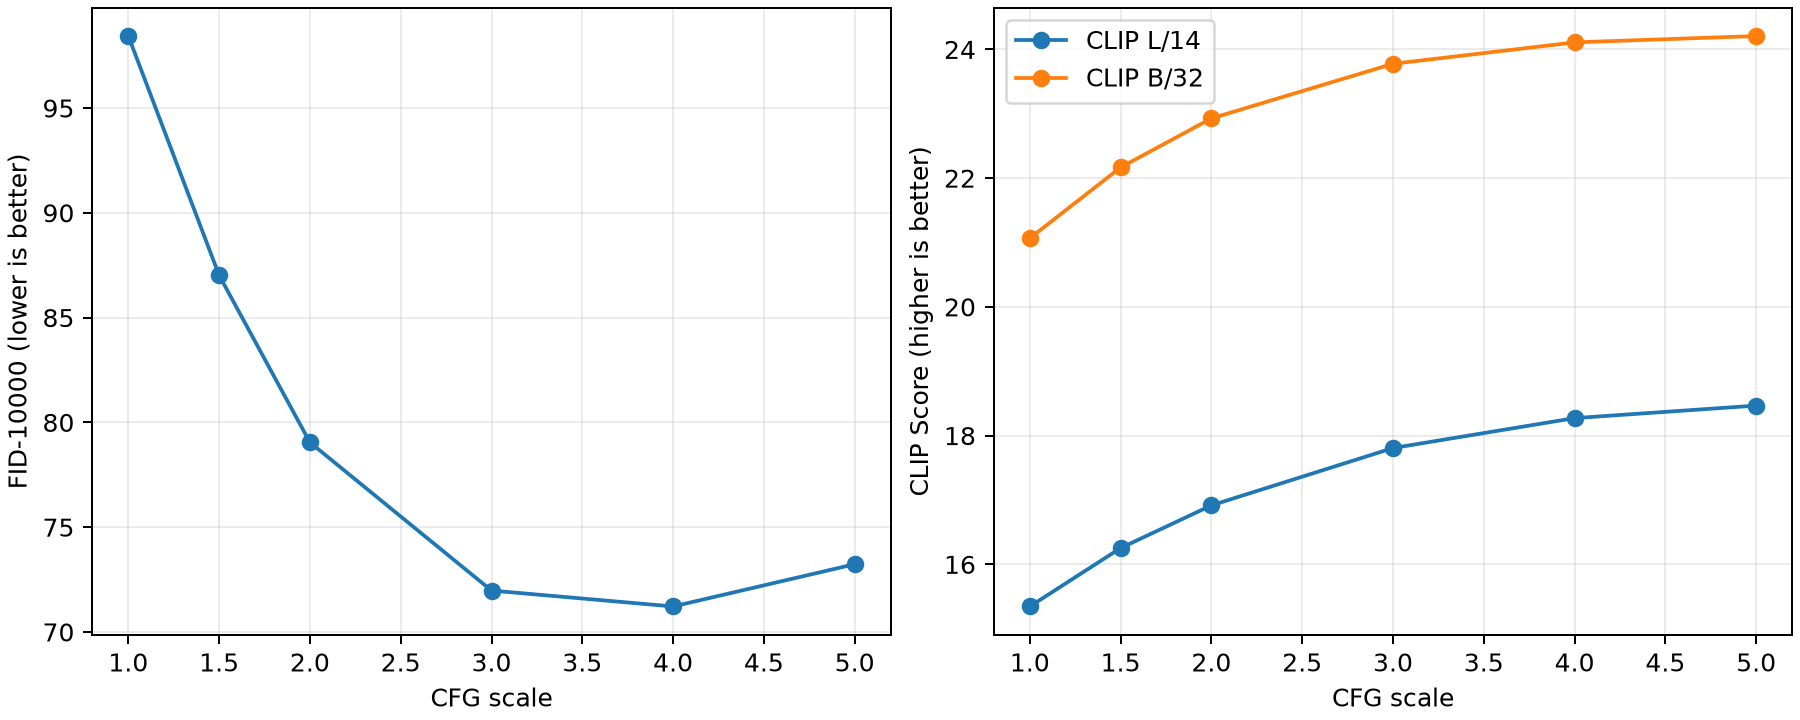
\includegraphics[width=0.92\textwidth]{outputs/evaluation/dit_s4_150k/figuras/cfg_metrics.png}
  \caption{FID-10K (left) and CLIP Score (right) as a function of the CFG scale $s$ (DPM-Solver++, 20 steps). The FID vs CLIP Score trade-off curve is shown in Appendix~\ref{app:figs}.}
  \label{fig:cfg}
\end{figure}

\paragraph{Real-image reference.}
On the same 10,000 image--caption pairs, real images obtain CLIP Scores of 25.5643 (L/14) and 30.1501 (B/32), against 18.2717 and 24.1091 for the generated images at DPM-Solver++ 20, $s=4$.
The real-image score is a practical reference, not a strict maximum: at this setting 9.3\% (L/14) and 11.7\% (B/32) of generated images score above their real counterpart.

\paragraph{Images with and without people.}
Of the 10K references, 5,250 have person annotations and 4,750 do not; the second group is used whole and the first is subsampled to 4,750 (Table~\ref{tab:groups}).
Real images obtain similar CLIP Scores in both groups, whereas generated images score higher and have a lower FID-4750 in the group with people.
A bootstrap over images (5,000 resamples, 95\% intervals), computed from the per-image scores, gives a generated-image difference (with minus without people) of 3.15 [3.02, 3.29] for L/14 and 3.65 [3.52, 3.79] for B/32.
These intervals cover only the choice of images for this one generated sample, not a new seed or a retrained model, and no interval exists for FID-4750.
The groups differ in content, captions and composition as well as in the presence of people, so this breakdown describes the gap but does not identify its cause.
The group means of CLIP Score and the group selection were recomputed from the stored per-image scores and match; FID-4750 and the per-image scores themselves were not recomputed in our review.

\begin{table}[t]
  \caption{Metrics for balanced groups of val2014 images with and without person annotations (DPM-Solver++ 20, $s=4$, center crop, $N=4{,}750$ per group). FID-4750 is comparable only between these two groups.}
  \label{tab:groups}
  \centering
  \small
  \begin{tabular}{@{}lrrrrr@{}}
    \toprule
     & & \multicolumn{2}{c}{CLIP L/14} & \multicolumn{2}{c}{CLIP B/32} \\
    \cmidrule(lr){3-4}\cmidrule(l){5-6}
    Group & FID-4750 & Generated & Real & Generated & Real \\
    \midrule
    With person annotations & 56.3083 & 19.7638 & 25.5768 & 25.8457 & 30.0862 \\
    Without person annotations & 116.3012 & 16.6117 & 25.5185 & 22.1943 & 30.2021 \\
    \bottomrule
  \end{tabular}
\end{table}

\paragraph{Degenerate outputs.}
All-black images appear only at $s\geq4$: 3 with DPM-Solver++ at $s=4$, 3 at $s=5$ and 7 with DDPM at $s=4$; 12 of these 13 belong to the group without person annotations.
Their rate is at most 0.07\%, too low to explain the overall FID, and their cause is unknown.

\subsection{Qualitative results}

Figure~\ref{fig:grid} shows the training grid at 150K.
The baseball prompt gives the clearest result: field, players and stands are recognizable, although the players are deformed.
The woman-on-bicycle prompt gives an outdoor park scene with a deformed figure and no clear bicycle, and the food prompt gives warm food-like colors and textures without a clear plate or table.
The remaining prompts reproduce only colors or textures related to the caption (sunset colors without a dog, blue sky with a blurred blob, dark purple forms) or are mostly dark with no recognizable subject.
Across the 50K, 100K and 150K grids, compositions stay similar and details change; this is one seed on 8 prompts and not a measure of convergence.

\begin{figure}[t]
  \centering
  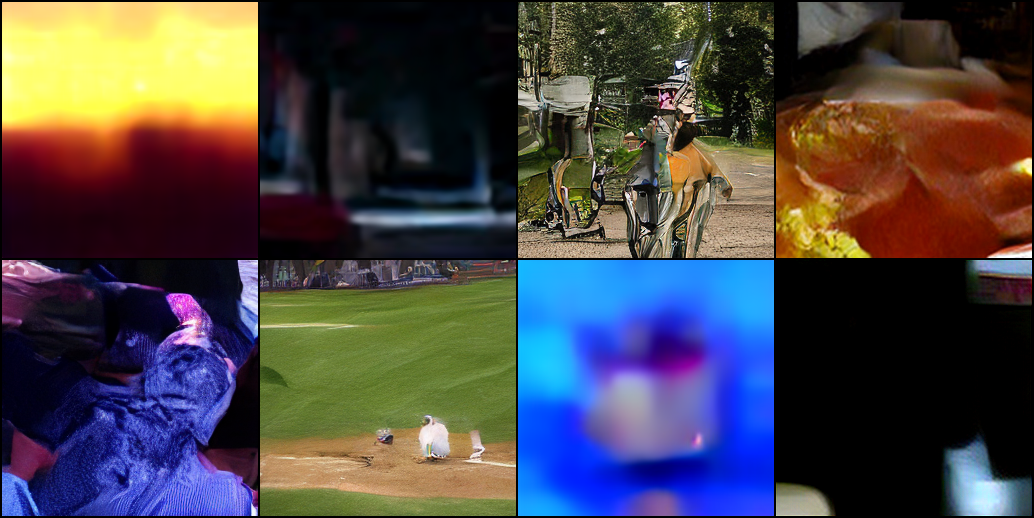
\includegraphics[width=0.85\textwidth]{outputs/training/samples/0150000.png}
  \caption{Training grid at step 150K (EMA, DPM-Solver++ 20 steps, $s=4$, seed 0). Top row: ``A dog sitting on a beach at sunset'', ``A red car parked in front of a building'', ``A woman riding a bicycle in a park'' and ``A plate of food on a wooden table''; bottom row: ``A cat sleeping on a couch'', ``A group of people playing baseball'', ``An airplane flying over mountains'' and ``A vase of flowers next to a window''.}
  \label{fig:grid}
\end{figure}

Figure~\ref{fig:examples} shows evaluation examples.
These are the first entries of the frozen evaluation manifest and were not selected for quality.
Across the eight stored examples, a man walking into the ocean gives a recognizable beach with a deformed figure and object; a bird among purple flowers gives colored regions without an identifiable bird; and a man and two women walking their dogs in the woods gives a wooded scene with deformed figures and no recognizable dogs.
The samples thus match categories and scenes in part, but fail on anatomy, object count and complex actions, and some high-$s$ images look blocky and oversaturated.
These are examples, not a global measure, and they do not show that one sampler looks better than the other.

\begin{figure}[t]
  \centering
  \setlength{\tabcolsep}{1pt}
  \begin{tabular}{cccc}
    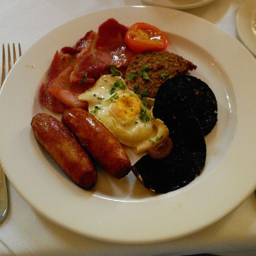
\includegraphics[width=0.22\textwidth]{outputs/evaluation/dit_s4_150k/muestras/000000434763/real.png} &
    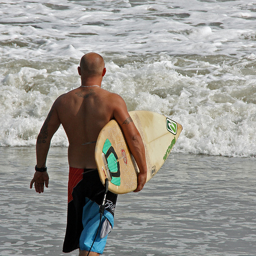
\includegraphics[width=0.22\textwidth]{outputs/evaluation/dit_s4_150k/muestras/000000332058/real.png} &
    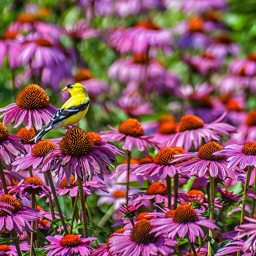
\includegraphics[width=0.22\textwidth]{outputs/evaluation/dit_s4_150k/muestras/000000117237/real.png} &
    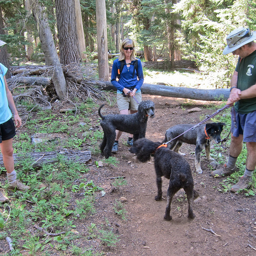
\includegraphics[width=0.22\textwidth]{outputs/evaluation/dit_s4_150k/muestras/000000057703/real.png} \\
    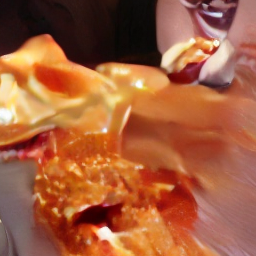
\includegraphics[width=0.22\textwidth]{outputs/evaluation/dit_s4_150k/muestras/000000434763/final_dpm_cfg_4.png} &
    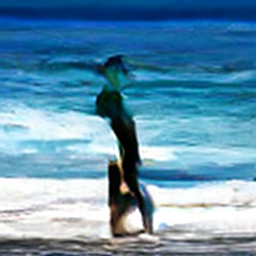
\includegraphics[width=0.22\textwidth]{outputs/evaluation/dit_s4_150k/muestras/000000332058/final_dpm_cfg_4.png} &
    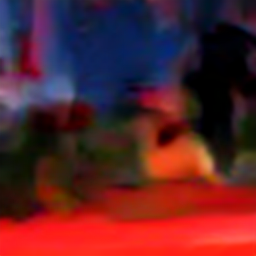
\includegraphics[width=0.22\textwidth]{outputs/evaluation/dit_s4_150k/muestras/000000117237/final_dpm_cfg_4.png} &
    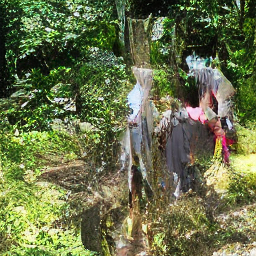
\includegraphics[width=0.22\textwidth]{outputs/evaluation/dit_s4_150k/muestras/000000057703/final_dpm_cfg_4.png} \\
    (a) & (b) & (c) & (d)
  \end{tabular}
  \caption{Real val2014 references (top, center crop) and generated images (bottom, DPM-Solver++ 20, $s=4$) for the first four entries of the evaluation manifest, not selected for quality. Captions: (a) ``A white plate with sausage, eggs and other meat.'', (b) ``A man walking into the ocean while holding a surfboard.'', (c) ``A bird sitting in a field of beautiful purple flowers.'', (d) ``A man and two women walking their dogs and hiking in the woods.''}
  \label{fig:examples}
\end{figure}

\subsection{Limitations}

\begin{itemize}
    \item \textbf{Reduced training data.} The run used only the 45,174 images with person annotations and five captions, out of the 82,783 planned, so the model saw a little over half (54.6\%) of the planned training images.
  \item \textbf{No hyperparameter search.} The computational cost of training ruled out a hyperparameter study. The hyperparameters were taken from the DiT paper, with a few adjusted to our setting, so the final run is not a tuned configuration.
  \item \textbf{One seed, one checkpoint.} All metrics come from one seed and the 150K checkpoint; FID-2K exists only at 150K, so there is no convergence curve and no claim about convergence can be made.
  \item \textbf{Null embedding.} $\nullemb$ is all zeros, not CLIP(\texttt{""}) as specified. The MLP maps it to a constant $\yemb$ that the model learns as ``no caption'', similar to DiT's learned null embedding.
  \item \textbf{Feature provenance.} The team member who ran the training reported that the features came from the final version of the extraction script, which stores unscaled statistics so that 0.18215 is applied once. This was not independently verified.
\end{itemize}

% ---------------------------------------------------------------------------
\section{Conclusions and future work}

We adapted DiT-S/4 from class-conditional to text-conditional generation by replacing the label lookup with an MLP over the frozen CLIP ViT-L/14 pooled embedding and feeding $c=\temb+\yemb$ to the unchanged DiT backbone.
On this checkpoint, evaluation set and seed, $s=4$ has the lowest FID-10K in the sweep (71.2168), CLIP Score rises with $s$ up to 5, DPM-Solver++ 20 has a lower FID-10K than DDPM 250 at $s=4$, and real-image CLIP Scores remain substantially higher than generated ones.
Image quality is limited: scenes and colors follow the caption in part, but objects, people and relations are not rendered correctly.
The run saw 18.8\% of the planned samples on a person-only subset, so these results do not show what the specified configuration would achieve.

Future work, in order of what it would clarify:
(i) an overfit test on 64 images to separate a code error from limited training;
(ii) FID-2K at the 50K and 100K checkpoints to see how results evolved;
(iii) an evaluation with the person crop at $s=4$, reported separately, to measure the model on its training crop;
(iv) a run following the specification (82,783 images, center crop, $\nullemb=\mathrm{CLIP}(\texttt{""})$, 400K steps);
(v) ablations of the text projection (MLP vs Linear), of $\nullemb$ (learned vs CLIP(\texttt{""})), of the guidance scale and of the sampler steps;
and (vi) a cross-attention variant over $E_{\mathrm{seq}}$, since global conditioning is expected to limit attribute binding and spatial relations.
Larger DiT configurations and smaller patches, which improve FID in the original paper~\cite{peebles2023dit}, are a further direction.

% ---------------------------------------------------------------------------
\small
\bibliographystyle{unsrt}
\bibliography{references}
\normalsize

% ---------------------------------------------------------------------------
\appendix
\section{Technical appendices}

\subsection{Full configuration of the final run}
\label{app:config}

\begin{table}[h]
  \centering
  \small
  \begin{tabular}{@{}ll@{}}
    \toprule
    Item & Value \\
    \midrule
    Model & DiT-S/4: depth 12, hidden 384, 6 heads, patch 4, 64 tokens, \texttt{learn\_sigma=True} \\
    Parameters & 33,003,776 (text embedder 443,136; incl.\ frozen positional embedding) \\
    Conditioning & adaLN-Zero-Text: CLIP ViT-L/14 $\epooled$ (768) $\to$ Linear--SiLU--Linear $\to$ 384 \\
    VAE & \texttt{sd-vae-ft-ema}, frozen, encode and decode, $f=8$, scale 0.18215 \\
    Text dropout & 0.15, replaced by $\nullemb$ \\
    $\nullemb$ & All-zero vector $(1,768)$, stored as a buffer in the checkpoint \\
    Data & 45,174 train2014 images with people; person crop at 256; original $+$ flip; 5 captions \\
    Optimizer & AdamW, lr $10^{-4}$, weight decay 0, no warmup, no gradient clipping \\
    Batch / length & 128 / 150,000 steps ($\approx$425 epochs), seed 0, 4 data workers \\
    Diffusion & $T=1000$, linear $\beta$ $10^{-4}\to0.02$, $t\in\{0,\dots,999\}$ \\
    Loss & Hybrid: $L_{\mathrm{simple}}+L_{\mathrm{vlb}}$ (code: \texttt{mse + vb}, no extra weight) \\
    EMA & 0.9999 \\
    Precision / hardware & bf16 autocast on the model forward; CPU, $\approx$2.0 steps/s, $\approx$21 h \\
    Logging & Every 100 steps: loss, MSE, vb, gradient norm \\
    Checkpoints and grids & Rolling checkpoint and grid every 10K steps; permanent every 50K \\
    Grid sampling & EMA, DPM-Solver++ 20 steps, $s=4.0$, seed 0, 8 fixed prompts \\
    Final logged values & Loss 0.1684, MSE 0.1614, vb 0.0071 at step 150,000 \\
    \bottomrule
  \end{tabular}
\end{table}

\paragraph{Checkpoint.}
\texttt{last.pt}, EMA weights at step 150,000, 528,048,707 bytes, SHA-256 \\
\texttt{f693fd7391979856e7059994643e755239276ba5d66a31becf1ebf1e18e93c6b}. \\
The state dict loads strictly, all weights are finite and $\|\nullemb\|=0$.

\paragraph{Software.}
Evaluation environment: torch 2.14.1, torchvision 0.29.1, timm 1.0.30, diffusers 0.35.2, transformers 4.57.6, torchmetrics 1.9.0, clean-fid 0.1.35.
The test suite (50 passed, 1 skipped for CUDA) was run with Python 3.11 in a clean environment.
The software versions of the training environment were not recorded.

\paragraph{VAE choice.}
\texttt{sd-vae-ft-ema} and \texttt{sd-vae-ft-mse} share the same encoder and differ only in the fine-tuned decoder; on COCO 2017 val at $256\times256$ the model card reports rFID 4.42 and PSNR 23.8 for ft-EMA, and rFID 4.70 and PSNR 24.5 for ft-MSE~\cite{stability_sdvae}.

\paragraph{Text encoding.}
The evaluation passes the attention mask to the CLIP text encoder and training does not. A test with a small, randomly initialized CLIP gave identical pooled outputs, since padding comes after [EOS]; the difference is therefore not a source of bias in this setting.

\subsection{Training curve}
\label{app:curve}

\begin{table}[h]
  \centering
  \small
  \begin{tabular}{@{}lrrrr@{}}
    \toprule
    Steps & Mean loss & Mean MSE & Mean vb & Mean grad norm \\
    \midrule
    100 (single log) & 0.5205 & 0.5084 & 0.0121 & 1.4020 \\
    100--10K & 0.1945 & 0.1868 & 0.0077 & 0.1358 \\
    10K--50K & 0.1775 & 0.1700 & 0.0075 & 0.0317 \\
    50K--100K & 0.1721 & 0.1646 & 0.0074 & 0.0229 \\
    100K--140K & 0.1697 & 0.1623 & 0.0074 & 0.0205 \\
    140K--150K & 0.1687 & 0.1614 & 0.0073 & 0.0199 \\
    \bottomrule
  \end{tabular}
\end{table}

The logged rates average 2.015 steps/s and add up to 20.9 h.

\subsection{Intermediate evaluation and verification}

FID-2K at 150K (DPM-Solver++ 20, $s=4$): 94.1912, CLIP Score 18.3290 (L/14) and 24.1158 (B/32). These values are not comparable with FID-10K; the same configuration gives 71.2168 with 10K images.
Sanity checks that were run: parameter count 33,003,776; output at initialization of shape $(2,8,32,32)$ and all zeros; measured text dropout 0.1501 ($N=100{,}000$); CFG output matching the manual formulation; and a replay of the evaluation with the stored generated images.
In the internal review of the evaluation, the code and stored traces were checked and no error was found; generation and FID were not re-run.

\subsection{Additional figure}
\label{app:figs}

\begin{figure}[h]
  \centering
  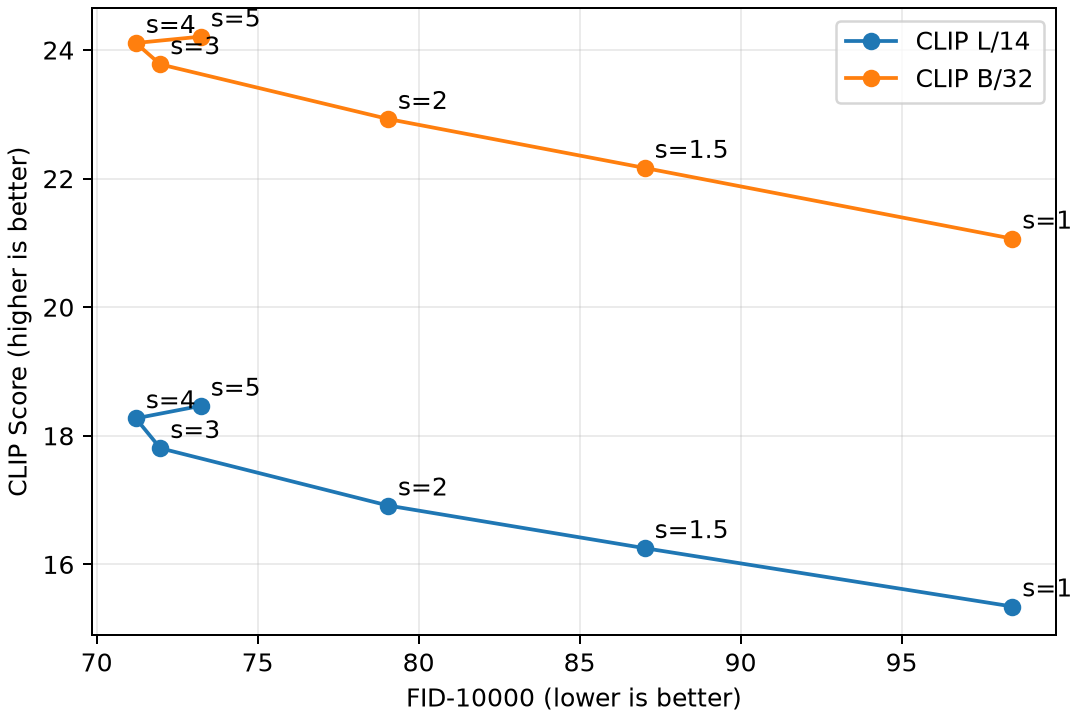
\includegraphics[width=0.6\textwidth]{outputs/evaluation/dit_s4_150k/figuras/fid_vs_clip.png}
  \caption{FID-10K vs CLIP Score across the CFG sweep (DPM-Solver++, 20 steps), for CLIP ViT-L/14 and ViT-B/32.}
  \label{fig:fidclip}
\end{figure}

% ---------------------------------------------------------------------------
\section*{Author Contributions}

Contributions are described using the CRediT taxonomy (\url{https://credit.niso.org/}).
\textbf{Linda Fei Payeras Olano:} Data curation; Software (feature extraction and dataset).
\textbf{Milagros Rodriguez Ventura:} Software (text-conditioned model, final clean-up and documentation of the repository); Validation (model tests).
\textbf{David L\'opez Valdivia:} Software (training script); Investigation (training run).
\textbf{Daniel Cruz Navarro:} Software (sampling and evaluation); Investigation (evaluation runs); Formal analysis (analyses of the results).

\section*{Declaration regarding the use of AI tools}

During the preparation of this manuscript, the authors used Claude for AI-assisted language editing, coding and literature support. The use of the tool was limited to writing the initial draft of the report and ensuring code quality and correctness. The authors independently verified the output and retain full responsibility for the accuracy, integrity, originality, and final content of the manuscript.

\end{document}
